\section{Overview}\label{subsec:overview}

This section starts by motivating the problem of boilerplate code in
traversals of complex structures. It then shows how \name addresses
the problem using a combination of object algebras~\cite{bruno12oa}
and Java annotations.


%Thus we introduce generic queries and transformations to make traversal code reusable and modular. Finally we present our framework \name which a%utomatically generate generic queries, generalized generic queries, transformations and contextual aware transformations based on Object Algebra Int%erfaces with Java annotation.

\subsection{A Company Structure and an Object Oriented Solution}

\begin{figure}[t]
\centering
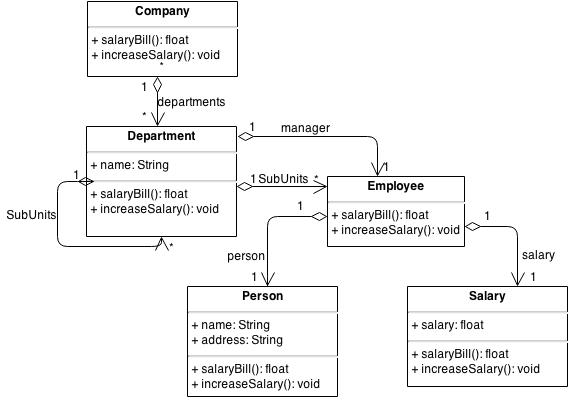
\includegraphics[width=110mm]{Company.jpg}
\caption{Company Structure \label{company_structure}}
\end{figure}

We start by considering the company structure introduced in
Figure~\ref{company_structure}. The example is inspired by L\"ammel
and Peyton Jones company structure, used to motivate their ``Scrap
your Boilerplate'' approach~\cite{ralf03syb}. It is also closely
related to the 101 companies system~\cite{Inauguration101}.

A very natural Object-Oriented way to model the company structure is
illustrated in Figure~\ref{oop_company}. A \lstinline{Company}
comprises a list of \lstinline{Department}s. Each
\lstinline{Department} is managed by an \lstinline{Employee},
and contains a list of \lstinline{SubUnits}. A
\lstinline{SubUnit} can be either a \lstinline{Department} or an
\lstinline{Employee}. An \lstinline{Employee} is a \lstinline{Person}
with an associated \lstinline{Salary} information.

\begin{figure}[tb]
\lstinputlisting[linerange=6-23]{../ObjectAlgebras/src/sybDemo1/Company.java} % APPLY:linerange=OOP_COMPANY
\vspace{-.1in}
\caption{The \lstinline{Company} and \lstinline{Salary} classes
  implementing part of the company structure.}
\label{oop_company}
\end{figure}

Two operations are supported by the company structure: querying the
salary bill for the whole company; and increasing the salary of each
employee by 10\%. To support those operations, a very natural OO
solution is to have methods \lstinline{salaryBill} and
\lstinline{increaseSalary} in all classes from the bottom
\lstinline{Salary} class to the top \lstinline{Company} class. Only in
sibling classes such as the \lstinline{Person} class, which has
nothing to do with salary information, the methods would be ommitted.

Figure~\ref{oop_company} shows the Java implementation of the  
\lstinline{Salary} and \lstinline{Company} classes. The implementation 
of other classes is ommitted for space reasons.
In the implementation, querying the salary bill of the whole company is done
by returning the salary in instances of the \lstinline{Salary} class,
and delegating the method \lstinline{salaryBill} to the child leaves
in other classes. Increasing the salary for the whole
company by 10\% can be implemented similarly. The salary information
in instances of the \lstinline{Salary} class is updated, and the
method \lstinline{increaseSalary} is delegated to the child leaves in
the other classes.\bruno{increaseSalary is mutating the company, but
  with OAs we create a new company.}

\begin{comment}
Just as in functional programming, modelling such company structure in
a conventional OO way leads to significant amounts of boilerplate
code. Object algebras provide an alternative way to model the company
structure, with benefits in terms of extensibility, but there is still
boilerplate code.
\end{comment}

However, this simple object-oriented solution has two important problems:

\begin{enumerate}

\item {\bf Lack of extensibility} The Object-Oriented style
  representation of data structures is cumbersome and
  inflexible due to the bound relationship between classes. For
  instance, adding a class \lstinline{Team} requires modifying the
  parent classes and child classes, and is also prone to errors.
  Adding a new operation such as pretty
  printing the company structure requires pervasive changes across all
  existing classes.

\item {\bf Boilerplate traversal code} Another issue is
  that we usually need to write a large amount of boilerplate code to
  implement traversals. In
  our example, we implemented \lstinline{increaseSalary} and
  \lstinline{querySalary} in almost all classes. However only the
  \lstinline{Salary} class does some interesting work. All other classes
  simply delegate the task to the child nodes. This problem becomes
  more severe with bigger tree structures. The interesting code can
  become a very small portion of the code needed to perform a
  traversal: most of the code is doing tedious
  walking of the structure.

\end{enumerate}

\subsection{Modeling the Company Structure with Object Algebras}

To tackle with the problem of extensibility, Object Algebras is a good solution. \bruno{text missing here. We need to introduce object algebras first; explain what they are; cite them; and then talk about the solution.} Oliveira proposed the design pattern \emph{Object Algebras}\cite{bruno12oa} to solve the famous Expression Problem. Object Algebras are classes that implement Object Algebra Interfaces where the type parameters represents the algebra classes. With this extra layer of generic type parameters, Object Algebras is extensible on both data variants and operations.  

\begin{figure}[tb]
\lstinputlisting[linerange=8-17]{../ObjectAlgebras/src/trees/SybAlg.java} % APPLY:linerange=SYB_TREE
\vspace{-.1in}
\caption{Company Structure represented by Object Algebra Interface}
\label{syb_tree}
\end{figure}

Fig.~\ref{syb_tree} shows the approach to model the Company
structure as an object algebra interface. Different operations can be realized by extending object algebras inheriting from the object algebra interface. To implement query bill
operation for the whole Company structure, we can pass in a \lstinline{Float} class to represent salary and implement the
Company interface with specific operation for each component. In our case, the \lstinline{QuerySalarySybAlg} returns salary information in method \lstinline{Float S(float salary)} and does the delegation work in most other methods related to salary information.

\begin{lstlisting}[numbers=none] 
public class QuerySalarySybAlg implements SybAlg<Float,Float,Float,Float,Float,Float> {
	public Float C(List<Float> depts){
		Float r = 0f;
		for (Float f: depts) r += f;
		return r;
	}
	...
	public Float S(float salary){
		return salary;
	}
}
\end{lstlisting}

IncreaseSalary will modify an old algebra and return a new algebra based on specific implementations. More specifically, the old algebra is set as a field in \lstinline{IncreaseSalarySybAlg}, method  \lstinline{Salary S(float salary)} increases the salary by 10\%, and other methods simply delegates to the same methods in the old algebra. 

\begin{lstlisting}[numbers=none]
public class IncreaseSalarySybAlg<Company, Dept, SubUnit, Employee, Person, Salary> implements SybAlg<Company, Dept, SubUnit, Employee, Person, Salary> {
	public SybAlg<Company, Dept, SubUnit, Employee, Person, Salary> alg;
	public IncreaseSalarySybAlg(SybAlg<Company, Dept, SubUnit, Employee, Person, Salary> alg) { this.alg = alg; }
	public Float C(List<Dept> depts) {
		return alg.C(depts);
	}
	...
	public Salary S(float salary) {
		return alg.S(salary*1.1f);
	}
}
\end{lstlisting}\bruno{The code is too specific. It should be
  something like: \lstinline{public class
    IncreaseSalarySybAlg<Company, Dept, SubUnit, Employee, Person,
    Salary> implements SybAlg<Company, Dept, SubUnit, Employee,
    Person, Salary>}}

\bruno{code needs to be better explained. What are we using the
  \lstinline{alg} for?}
  
When programming with Object Algebras, the code can be very generic based on the object algebra interfaces. \lstinline{alg} can be used as an abstract factory to construct algebras, while the algebras can be instantiated by specific object algebras later by passing in type parameters. 

However, although we solved the problem of extensibility with object algebras, the traversal code is still lengthy and we are still writing tedious traversing code of tree structures. The only code we are really interested in is the \lstinline{Salary S(Float salary)} method to return or to increase the salary. It will be better if we can design some generic classes for queries and transformations. Hence specific algebras can be generated by
implementing interesting cases of generic queries and
transformations. Moreover, it will be even better if the boilerplate code can be generated automatically so we can focus our attention on the interesting cases.

\subsection{Object Algebra Framework}
Motivated by this problem of writing generic code for tree structure
traversals, we introduce generic queries, generalized generic queries, transformations and contextual aware transformations with Object Algebras, which can be easily inherited by real cases of queries and transformations. Furthermore, we designed an object algebra framework \name. With our framework, the generic query and transformation classes can be generated automatically by adding an ``$@$Algebra'' annotation.

Now with our Object Algebra Framework, the code we need to write for Salary Bill and Increase Salary will be much shorter. A Generic query code will be as short as Fig.~\ref{query_with_oaframework}. Here when coding with the framework \name, users need not worry about any boilerplate delegation code of the tree structure, but just simply rewrite the interesting case which actually return the salary information.
\begin{figure}[tb]
\lstinputlisting[linerange=8-11]{../ObjectAlgebras/src/example_SybAlg/FloatQuery.java} % APPLY:linerange=QUERY_WITH_OAFRAMEWORK
\vspace{-.1in}
\caption{Query Salary Class with Object Algebra Framework}
\label{query_with_oaframework}
\end{figure}

Transformation code will be like Figure~\ref{transform_with_oaframework}. Similar to the query example, all the boilerplate part has been handled by the framework and the developer only needs to pass in the original company algebra and override the interesting case \lstinline{Float S(float salary)}, then a new company algebra will be returned after transformation.  
\begin{figure}[tb]
\lstinputlisting[linerange=7-12]{../ObjectAlgebras/src/example_SybAlg/IncSalary.java} % APPLY:linerange=TRANSFORM_WITH_OAFRAMEWORK
\vspace{-.1in}
\caption{Increase Salary Class with Object Algebra Framework}
\label{transform_with_oaframework}
\end{figure}

\bruno{code is too specific. See comment about previous
  increase salary example}
\begin{comment}The classes SybAlgQuery<R>, SybAlgTransform<R,R,R,R,R,R> are generated
by the framework automatically. \end{comment}
\bruno{Jason, generally speaking your explanations of the code are to
  brief: you don't actually explain the code. You need to emphasize
  the relevant parts of the code, as well as the parts that are
  non-obvious. Here for example you want to emphasize that we only
  need to write the salary method.}
